\documentclass[a4paper]{article}
\usepackage{geometry}
\usepackage{fullpage} % Package to use full page
\usepackage{parskip} % Package to tweak paragraph skipping
\usepackage{tikz} % Package for drawing
\usepackage{tikz-qtree}
\usepackage{amsmath}
\usepackage{hyperref}
\usepackage[utf8]{inputenc}
\usepackage{lmodern}
\usepackage[MeX]{polski}
\usepackage{amssymb}

\title{Notatki z baz danych}
\author{Małgorzata Dymek}
\date{}

\newgeometry{tmargin=1.5cm, bmargin=1.5cm, lmargin=1.2cm, rmargin=1.2cm}

\begin{document}

\maketitle
\section{Podstawowe pojęcia}

\textbf{Baza danych} -  kolekcja powiązanych ze sobą danych.
\begin{itemize}
    \item Reprezentuje pewne \textbf{aspekty świata rzeczywistego} (mini świat) lub obszar analizy, czasem dziedzinę problemu.
    \item Jest \textbf{logicznie spójnym zbiorem} danych o pewnym znaczeniu.
    \item Stworzona \textbf{w określonym celu}, dla pewnej grupy użytkowników.
\end{itemize}

\textbf{Logika biznesowa} -  implementacja \textbf{procesów biznesowych}.\\

\textbf{System Zarządzania Bazą Danych (SZBD)} - system oprogramowania, który zapewnia: 
\begin{itemize}
    \item definiowanie, tworzenie, utrzymywanie bazy danych.
    \item operowanie na danych, kontrolę \textbf{spójności}, dbanie o \textbf{integralność}.
    \item odporność na błędy, \textbf{mechanizmy bezpieczeństwa}, kontrola dostępu.
    \item udostępnianie \textbf{metadanych}, dostępność przez różne interfejsy, komunikacja z innymi systemami.
    \item obsługa transakcji (ACID), sterowanie współbieżnością.
\end{itemize} 

\textbf{System bazy danych (SBD) - bazy + SZBD}. Czasami zalicza się również aplikację użytkowników.\\

\textbf{Relacyjne systemy baz danych}
\begin{itemize}
    \item \textbf{Niezależność} między danymi a programami.
    \item \textbf{Samoopisujący charakter SZBD} – zawiera \textbf{meta-dane}.
    \item Dostarczanie \textbf{wielu widoków}  tych samych danych dla różnych użytkowników.
    \item Zapewnienie \textbf{integralności} danych.
    \item Współdzielenie danych, \textbf{przetwarzanie współbieżnych transakcji} wielu użytkowników.
    \item Wysoka \textbf{niezawodność i bezpieczeństwo}.
    \item Generalnie relacyjne systemy baz danych \textbf{źle się skalują poziomo}.
\end{itemize}
\hfill \\\\\\
\textbf{Bazy danych NoSQL}
\begin{itemize}
    \item Gromadzenie i \textbf{szybkie przetwarzanie} dużych ilości danych.
    \item Stosunkowo \textbf{łatwe skalowanie poziome}.
    \item Często: \textbf{struktura rozproszona}.
    \item Często: brak schematu określonego na poziomie samego systemu baz danych (ale schemat jest często narzucany przez aplikacje klienckie).
    \item Na ogół: \textbf{brak lub niepełna obsługa transakcji}.
\end{itemize}

\subsection{Architektury systemów baz danych}

\subsubsection{Trójwarstwowa architektura ANSI-SPARC}
\begin{itemize}
    \item \textbf{Warstwa zewnętrzna} - dostarcza \textbf{niezależne, spersonalizowane widoki} użytkownikom. Użytkownicy nie muszą mieć dostępu do szczegółów.
    \item \textbf{Warstwa konceptualna} - dostarcza \textbf{jednolitego, globalnego widoku} danych i ich wzajemnych powiązań. Jest \textbf{niezależna od użytkowników}. Dostęp do niej mają zazwyczaj administratorzy.
    \item \textbf{Warstwa wewnętrzna} -  opisuje jak dane są \textbf{fizycznie przechowywane}.
\end{itemize}
Zmiany wewnątrz warstwy niekoniecznie naruszają pozostałe.

\subsubsection{Architektury komunikacyjne klient-serwer}
\begin{itemize}
    \item \textbf{Architektura dwuwarstwowa} - logika biznesowa w kliencie bądź serwerze bądź podzielona.
    \item \textbf{Architektura trójwarstwowa} - logika biznesowa w warstwie środkowej, na serwerze aplikacji.
    \item \textbf{Architektury wielowarstwowe} - wyspecjalizowane warstwy.
\end{itemize}

\subsection{Modelowanie danych}
\begin{itemize}
    \item \textbf{Modele konceptualne} -  umożliwiają opis konkretnego, \textbf{wybranego wycinka rzeczywistości} poprzez analizę obiektów i powiązań między tymi obiektami.
    \item \textbf{Modele implementacyjne} - organizują struktury danych (modele relacyjne, obiektowo-relacyjne, obiektowe, No-SQL).
\end{itemize}

\subsubsection{Koncepcyjny model związków encji E/R}
\begin{itemize}
    \item \textbf{Encja} -  \textbf{jednostka} odpowiadająca „obiektowi” (zbiorowi obiektów).
    \item \textbf{Atrybut} – \textbf{cecha} encji.
    \item \textbf{Związek} - \textbf{zależność} między encjami.
\end{itemize}

\section{Relacyjne bazy danych}
Systemy oparte o model relacyjny.
\begin{itemize}
    \item Dane w \textbf{tabelach}. Tabela może przedstawiać \textbf{relację bazodanową}. 
    \item \textbf{Wiersz (rekord)} - dane reprezentujące pewną \textbf{encję lub związek}. Powinny być \textbf{unikalne} wewnątrz tabeli.
    \item \textbf{Atrybuty} - \textbf{kolumny}. Są nazwane i mają określony logicznie niepodzielny typ danych związany z dziedziną atrybutu.
    \item \textbf{Skalar} - pojedyncza wartość, najmniejsza semantycznie jednostka danych. Są \textbf{atomowe w ramach modelu} relacyjnego.
    \textbf{Dziedzina} to \textbf{zbiór wartości skalarnych}.
    \item \textbf{Zmienna relacji} - \textbf{nazwany obiekt, którego wartość zmienia się w czasie}. \textbf{Wartość  zmiennej} w danej chwili nazywa się \textbf{wartością relacji}.
    \item Relacyjna baza danych to \textbf{zestaw znormalizowanych relacji różnych stopni}. 
    \item Relacyjny model ma \textbf{zastosowanie na zewnętrznym i pojęciowym poziomie}, nie na wewnętrznym.
\end{itemize}

\subsection{Definicja Relacji wg Date'a}
Relacja R (w znaczeniu \textbf{wartość relacji}) na zbiorze niekoniecznie różnych dziedzin $D_1, D_2,\dots, D_n$ składa się z dwóch części: \textbf{nagłówka} (heading) i
\textbf{treści} (body).\\

\textbf{Nagłówek} jest to ustalony \textbf{zbiór atrybutów}, a ściśle rzecz biorąc zbiór par $<nazwa\_atrybutu : nazwa\_dziedziny>$, takich, że każdy unikalny atrybut odpowiada dokładnie jednej wyjściowej dziedzinie. Atrybuty \textbf{nie są uporządkowane}.\\

\textbf{Treść} jest to \textbf{zbiór krotek}. Każda krotka jest zbiorem par $<nazwa\_atrybutu : wartosc\_atrybutu>$. W każdej takiej krotce jest jedna para dla każdego atrybutu z nagłówka. Krotki są \textbf{unikalne, nieuporządkowane} oraz \textbf{istnieje przynajmniej jeden klucz kandydujący}.\\

Tak zdefiniowana relacja jest też określana terminem \textbf{relacja bazodanowa}.

\textbf{Liczebność} relacji - liczba krotek w zbiorze.\\
\textbf{Stopień relacji} - ilość dziedzin.\\

\subsection{Rodzaje relacji}
\begin{itemize}
    \item \textbf{Relacja nazwana} jest \textbf{nazwaną zmienną relacji} zdefiniowana w SZBD (CREATE TABLE/VIEW).
    \item \textbf{Relacja podstawowa} (autonomiczna) - wystarczająco ważna, by stanowić \textbf{nazwany niezależny byt} w bazie danych. "Przechowuje dane”.
    \item \textbf{Relacja wyprowadzana} (pochodna) - relacja, którą można otrzymać ze zbioru nazwanych relacji za pomocą jakiegoś \textbf{wyrażenia relacyjnego}.
    \item \textbf{Perspektywa} (widok) - \textbf{nazwana relacja pochodna}.Są \textbf{wirtualnymi zmiennymi} relacji.
    \item \textbf{Migawka} (perspektywa znormalizowana, snapshot) - \textbf{rzeczywista nazwana relacja pochodna}.
    \item \textbf{Wynik zapytania} - \textbf{nietrwała, nienazwana relacja pochodna} powstająca w wyniku realizacji \textbf{zapytania}.
    \item \textbf{Wynik pośredni} - \textbf{nietrwała, nienazwana relacja pochodna}, która powstaje w wyniku realizacji \textbf{podzapytania}.
\end{itemize}
\hfill \\
\textbf{Predykat} - rodzaj założenia pilnujący, żeby baza zawierała \textbf{dane zgodne z rzeczywistością}.

\subsection{Klucze}
\textbf{Klucz kandydujący} (potencjalny) w relacji R jest podzbiorem K (zbioru atrybutów relacji R), mającym:
\begin{itemize}
    \item \textbf{Własność jednoznaczności} - żadne dwie różne krotki z R nie mają tej samej wartości dla atrybutów z K.
    \item \textbf{Własność nieredukowalności} - żaden właściwy podzbiór K nie ma własności jednoznaczności. 
\end{itemize}

\textbf{Nadklucz/zbiór identyfikujący} - zbiór atrybutów posiadający \textbf{własność jednoznaczności}.

\textbf{Klucz złożony} - więcej niż jeden atrybut, \textbf{prosty} - jeden atrybut.

\textbf{Relacja może mieć więcej niż jeden klucz kandydujący. } Jeden z nich powinien być wybrany jako \textbf{klucz główny}. Reszta to \textbf{klucze alternatywne}.\\

\subsection{Problem integralności referencyjnej}
\textbf{Reguła integralności referencyjnej} - w bazie danych nie mogą występować żadne niedopasowane wartości kluczy obcych. Wchodzi ona w skład modelu relacyjnego danych. \textbf{Każdy stan} (wartości przechowywanych danych), \textbf{który nie spełnia tej reguły jest z definicji niepoprawny}.\\
\textbf{Więzy referencyjne} - warunki utrzymania integralności referencyjnej.\\

Sposoby \textbf{rozwiązania} problemu \textbf{stanów niepoprawnych}:
\begin{itemize}
    \item \textbf{ON DELETE/UPDATE RESTRICT} - niedopuszczenie do utworzenia niepoprawnych wartości.
    \item \textbf{ON DELETE/UPDATE CASCADE} - kaskadowe kasowanie lub aktualizowanie wartości tak, by zapewnić integralność referencyjną.
\end{itemize}

\subsection{Schematy relacji}
\textbf{Schemat relacji} - \textbf{zbiór atrybutów}, ozn. $R(A_1,A_2, \dots ,A_n)$. Ewentualnie zbiór atrybutów i zbiór wszystkich reguł integralności danych.\\
\textbf{Schemat relacyjnej bazy danych} S jest \textbf{zbiorem schematów relacji}, $S=\{ R_1, R_2, \dots , R_m \}$ wraz ze zbiorem wszystkich \textbf{więzów integralności} danych.

\subsection{Zależności funkcyjne}
\textbf{Wartość danej relacji} - definicja:

Niech R wartość relacji, X i Y dowolne podzbiory atrybutów R. Mówimy, że \textbf{Y jest funkcyjnie zależny od X} (ozn. $X \rightarrow Y$) wtw gdy: \\
jeśli dwie krotki z R mają \textbf{takie same wartości wszystkich atrybutów z X}, to mają również \textbf{takie same wartości wszystkich atrybutów ze zbioru Y}.\\\\
Przykład:
$\{PESEL\} \longrightarrow \{Nazwisko, Imie\}$\\

\textbf{Rodzaje zależności funkcyjnych}\\
Niech $A = \{A_1, A_2,\dots, A_n\},$ $B = \{B_1, B_2, \dots, B_m\}$ będą zbiorami atrybutów pewnej relacji.\\
\textbf{Zależność funkcyjna} jest:
\begin{itemize}
    \item \textbf{trywialna}, jeśli $B \subset A$.
    \item \textbf{nietrywialna}, jeśli $\exists b \in B : b \notin A$.
    \item \textbf{całkowicie nietrywialna}, jeśli $A \cap B =$  \O.
\end{itemize}

Zależność funkcyjna pojedynczego atrybutu od zbioru atrybutów - \textbf{nietrywialna}, jeśli atrybut z prawej strony nie należy do zbioru atrybutów z lewej strony. W zależności funkcyjnej zbiór wartości atrybutów z prawej strony jest zawsze zbiorem jednoelementowym.\\

\subsection{Zależności wielowartościowe}
Mówimy, że zbiór atrybutów $Y=\{Y_1, \dots ,Y_n\}$ schematu relacji R jest \textbf{wielowartościowo zależny} ($ X \twoheadrightarrow Y$ ) od zbioru atrybutów $X=\{X_1,\dots,X_m\}$, jeśli dla każdej pary krotek t i u, które mają takie same wartości atrybutów ze zbioru X, można znaleźć w tej instancji relacji krotkę w, której składowe mają wartości równe:
\begin{itemize}
    \item wartościom atrybutów ze zbioru X w krotkach t oraz u,
    \item wartościom atrybutów ze zbioru Y krotki t,
    \item wartościom tych składowych krotki u, które nie należą ani do X, ani do Y.
\end{itemize}

Niech X, Y, Z będą niepustymi zbiorami atrybutów, niech schemat relacji R będzie sumą tych zbiorów. Zależność $X \twoheadrightarrow Y$ zachodzi wtw, gdy zachodzi również $X \twoheadrightarrow Z$. ( $X \twoheadrightarrow Y | Z$ )\\

Zależność wielowartościową X ->> Y określa się jako \textbf{trywialną}, jeśli:
\begin{itemize}
    \item $Y \subset X$,
    \item $X \cup Y$ zawiera wszystkie atrybuty relacji.
\end{itemize}
\hfill \\
\textbf{Każda zależność funkcyjna jest zależnością wielowartościową}.\\

\textbf{Twierdzenie Fagina}\\
Niech X, Y, Z będą niepustymi zbiorami atrybutów, niech schemat relacji R będzie sumą tych zbiorów. Wówczas relacja jest \textbf{równa złączeniu swoich rzutów} na \{X, Y\} oraz \{X, Z\} wtw, gdy w relacji \textbf{zachodzi zależność wielowartościowa} $X \twoheadrightarrow Y | Z$.

\section{Projektowanie tabel}
Analiza rzeczywistości $\rightarrow$
Model związków encji ER $\rightarrow$
Diagram związków encji ERD

\textbf{Zasady projektowania tabel}
\begin{itemize}
    \item Każda \textbf{tabela} (relacja) ma \textbf{jednoznaczną nazwę}. Porządek w tabeli nie jest istotny. Powinna przechowywać informacje o \textbf{obiektach jednego rodzaju}.
    \item Każda \textbf{kolumna} (atrybut) ma \textbf{jednoznaczną nazwę, unikalną} w obszarze tabeli. Zawiera wartości \textbf{skalarne} jednego określonego \textbf{typu}.
    \item \textbf{Wiersze} są \textbf{unikalne}.
    \item W tabeli powinien istnieć (\textbf{klucz główny}).
    \item Unikanie redundancji.
\end{itemize}

\textbf{Anomalia wstawiania} - nie można wprowadzić nowej wartości, bo nie istnieje inna powiązana z nią ( np. nowego działu bez pracownika, jeśli informacja o działach jest w tabeli pracownicy).
\\
\textbf{Anomalia usuwania} - usunięcie jakiejś danej powoduje usunięcie innej (usunięcie wszystkich pracowników działu usuwa dział).\\

\subsection{Dekompozycja relacji} 
Rodzielenie tabeli opisującej obiekty wielu rodzajów na pojedyncze tabele obiektów jednego rodzaju.\\

Niech relacja R ma zbiór atrybutów $\{A_1,\dots, A_n\}$. Relację R dekomponujemy na relację S o schemacie $\{B_1, \dots , B_m\}$ oraz relację T o schemacie $\{C_1, \dots, C_k\}$ tak, by spełnione były następujące zasady:
\begin{itemize}
\item $\{A_1, \dots , A_n\} = \{B_1, \dots , B_m\} \cup \{C_1, \dots , C_k\}.$
\item Krotki S powstają przez rzutowanie wszystkich krotek relacji R na zbiór atrybutów $\{B_1, \dots , B_m\}$.
\item Analogicznie krotki T na zbiór atrybutów $\{C_1, \dots, C_k\}$
\end{itemize}
\hfill \\
\textbf{Odzyskiwanie danych po dekompozycji}\\
Chcemy, by w wyniku dekompozycji była możliwość takiego połączenia krotek powstałych w wyniku rzutowania, aby uzyskany zbiór krotek zawierał wszystkie i tylko te krotki, które
należały do relacji przed dekompozycją.\\
Jeśli mamy $\{A,B,C\}$ i $\{A \rightarrow B\}$, $\{B\rightarrow C\}$ zależności funkcyjne to odtworzymy, jeżeli tylko $A \rightarrow B$ to niekoniecznie.

\section{Normalizacja, postaci normalne}
Poziomy normalizacji relacji:
\begin{itemize}
    \item 1NF
    \item 2NF
    \item 3NF
    \item BCNF
    \item 4NF
    \item 5NF
    \item DKNF
\end{itemize}
W praktyce w większości przypadków doprowadzenie do 3NF usuwa redundancję i relacja już jest w wszystkich 'wyższych' postaciach. Absolutnym minimum jest 2PN lub 3PN.\\
Są systemy z nieznormalizowanymi tabelami, np. systemu analityczne, gdzie redundancja nie jest tak niekorzystna, ważniejsze są jakieś zestawienia danych, o spójność dbają systemy relacyjne (z normalizacją) dostarczające te dane.


\subsection{Pierwsza postać normalna}
\begin{itemize}
    \item Krotki są \textbf{unikalne, nieuporządkowane} oraz \textbf{istnieje przynajmniej jeden klucz kandydujący}.
    \item Atrybuty \textbf{nie są uporządkowane}, są \textbf{atomowe}.
    \item Wartości atrybutów są skalarne.
    \item Brak atrybutów cyklicznych, ew. gdy jesteśmy pewni dokładnej ilości danego atrybutu.
\end{itemize}
Relację spełniającą taki warunek nazywa się relacją
\textbf{znormalizowaną}.

\subsection{Druga postać normalna}
\textbf{Każdy atrybut wtórny jest w pełni zależny funkcyjnie od klucza kandydującego.}
Żaden niekluczowy (wtórny) atrybut nie jest zależny funkcyjnie od żadnego podzbioru właściwego klucza kandydującego.\\

Jeśli \textbf{wszystkie klucze} kandydujące są \textbf{proste} to relacja jest w \textbf{2PN}.

\subsection{Trzecia postać normalna}
\begin{itemize}
    \item Dla każdej nietrywialnej zależności funkcyjnej $\{A_1,\dots,A_n\} \rightarrow \{B\}$ zbiór atrybutów $\{A_1,\dots,A_n\}$ jest nadkluczem lub atrybut B jest elementem pewnego klucza kandydującego.
    \item \textbf{Żaden atrubyt niekluczowy nie jest zależny funkcyjnie od innego atrybutu niekluczowego}.
\end{itemize}

\textbf{Dekompozycja do 3PN}
\begin{itemize}
    \item Szukamy wszystkich nietrywialnych, całkowitych zależności funkcyjnych $\{A_1,\dots,A_n\} \rightarrow \{B_i\}$, które naruszają warunek trzeciej postaci normalnej. 
    \item Załóżmy, że otrzymujemy zależność (*)$\{A_1,\dots,A_n\} \rightarrow \{B_1, \dots, B_m\}$. Dzielimy schemat relacji na dwa nierozłączne podzbiory:
    \begin{itemize}
        \item Pierwszy, zawierający wszystkie atrybuty występujące w zależności (*).
        \item Drugi, zawierający atrybuty z lewej strony rozważanej zależności (*) oraz atrybuty nie występujące ani z lewej ani z prawej strony tej zależności. 
    \end{itemize}
\end{itemize}

\subsection{Postać normalna Boyce'a-Codda PNBC, BCNF}
\begin{itemize}
    \item Dla każdej całkowicie nietrywialnej zależności funkcyjnej $A \rightarrow B$ zbiór \textbf{A jest nadkluczem}.
    \item Każda relacja binarna jest w BCNF.
\end{itemize}
\hfill \\
\textbf{Dekompozycja do postaci BCNF} - jak dekompozycja do 3PN. \textbf{Nie zawsze zachowuje zależności funkcyjne}.

\subsection{Czwarta postać normalna}
Relacja jest w 4PN, jeśli dla każdej nietrywialnej zależności
wielowartościowej X ->> Y \textbf{zbiór X zawiera klucz relacji}.\\
\textbf{Dekompozycja do 4PN analogicznie}.

\subsection{Piąta postać normalna}

\subsubsection{Warunek 3D (3-rozkładalności)}
Rozważmy relację R o schemacie $\{P, C, W\}$. Jeśli wartość $p_1$ wiąże się z $c_1$, a $c_1$ wiąże się z $w_1$ oraz $w_1$ wiąże się z $p_1$, to $p_1$, $c_1$ i $w_1$ muszą występować w tym samym wierszu.\\
Uogólnienie do n-rozkładalności – relacja jest n-rozkładalna, gdy spełnia kilka takich cyklicznych warunków.\\

Warunek 3D jest spełniony wtw, gdy \textbf{relacja jest równa złączeniu trzech pewnych swoich rzutów}.

\subsubsection{Zależność złączenia}
Niech R będzie relacją, \{A, B, \dots, Z\} będą dowolnymi podzbiorami właściwymi zbioru atrybutów R. Mówimy, że relacja \textbf{R spełnia zależność złączenia} ozn. *( A, B, ..., Z ) wtw, gdy \textbf{R jest równa złączeniu naturalnemu swoich rzutów na \{A, B, ..., Z\}}.\\

\textbf{Zależność złączenia} *( A, B, ..., Z ) w relacji \textbf{wynika z zależności atrybutów schematu tej relacji od klucza} wtw, gdy \textbf{złączenia} naturalne rzutów są \textbf{realizowane względem} (pewnych) \textbf{kluczy} kandydujących relacji (\textbf{jest implikowana kluczami}).

\subsubsection{Piąta postać normalna}
Mówimy, że relacja jest w 5PN wtw, gdy \textbf{każda zależność złączenia w relacji jest implikowana kluczami kandydującymi} tej relacji.\\
Fagin udowodnił, że dowolna relacja może być bezstratnie zdekomponowana na równoważny zestaw relacji w piątej postaci normalnej (\textbf{postać 5NF jest zawsze osiągalna}).

\subsection{Postać normalna klucza dziedziny DKNF}
\textbf{Wszystkie więzy i zależności, które powinny być zachowane w poprawnych stanach relacji, mogą być wymuszane przez wymuszanie więzów domenowych oraz więzów kluczy na relacji}. Tylko związki wyrażane za pomocą kluczy obcych.\\
W praktyce użyteczność DKNF jest problematyczna, gdyż określenie w ten sposób różnych więzów może się okazać bardzo trudne.

\subsection{Denormalizacja}
W pewnych przypadkach projektant godzi się na doprowadzenie np. tylko do 2PN, mimo że występuje nadal redundancja. Nazywa się to \textbf{denormalizacją}. Może być korzystna ona z uwagi na \textbf{większą wydajność wyszukiwania}, bo złączenie tabel może być kosztowne. Jednak i tak nie powinno się tego robić.

\section{Transakcje}
\subsection{Wymagania (ACID)}
\begin{itemize}
    \item \textbf{Atomicity} (niepodzielność) transakcja jest wykonywana \textbf{w całości albo wcale}.
    \item \textbf{Consistency} (spójność) po zakończeniu transakcji baza musi być w stanie spójnym, tzn muszą być \textbf{zachowane wszystkie więzy} narzucone na dane.
    \item \textbf{Isolation} (izolacja) wykonywana w \textbf{izolacji od innych} transakcji.
    \item \textbf{Durability} (trwałość) po zakończeniu transacji jej \textbf{efekty} muszą być \textbf{trwałe} w systemie nawet w przypadku awarii.
\end{itemize}

\subsection{Stany transakcji}
\begin{itemize}
    \item \textbf{Aktywna} – podczas wykonywania operacji.
    \item \textbf{Częściowo zatwierdzona} – ostatnia operacja transakcji została wykonana. Teraz protokół zatwierdzania musi zapewnić \textbf{trwałość zmian}. Ew. sprawdzenie czy może zostać zatwierdzona. Jeśli może, to osiągnęła swój \textbf{punkt zatwierdzenia}.
    
    \item \textbf{Nieudana} – wykonywanie transakcji \textbf{nie może być kontynuowane}.
    
    \item \textbf{Przerwana, wycofana} – baza jest \textbf{odtworzona} do stanu sprzed rozpoczęcia transakcji.
    \item \textbf{Zatwierdzona} – wszelkie \textbf{zmiany} wykonane przez transakcje muszą być \textbf{trwałe}. Zatwierdzonej transakcji \textbf{nie można już wycofać} (ew. \textbf{transakcja kompensująca}).
\end{itemize}

\subsection{Implementacja atomowości i trwałości}
\textbf{Strategie zarządców buforów}

\begin{itemize}
    \item \textbf{Fix} - nie może być zapisów przed końcem transakcji.
    \item \textbf{No-Fix} - mogą być zapisy przed końcem transakcji. Synchronizacja może być realizowana \textbf{cyklicznie} w ramach procesu zwanego \textbf{punktem kontrolnym}.\\
    
    \item \textbf{Flush} - synchronizacja zmienionych bloków po zakończeniu transakcji. 
    \item \textbf{No-Flush} - brak obowiązku synchronizowania zmienionych bloków na koniec transakcji. Synchronizacja może być wykonana później.
\end{itemize}
W większości relacyjnych systemów baz danych, wykorzystujących tzw. \textbf{dzienniki transakcji} stosowana jest \textbf{strategia No-Fix/No-Flush}.

\subsection{Dziennik transakcji}
\begin{itemize}
    \item Zawiera \textbf{informacje o wszystkich wprowadzonych przez transakcje zmianach}.
    \item Mogą pojawić się informacje o operacji kompensującej, dane dotyczące operacji odczytu.
    \item Transakcja nie zostaje uznana za zakończoną, dopóki fizycznie na dysku w pliku dziennika nie znajdą się wpisy opisujące wszystkie przeprowadzone przez transakcję zmiany oraz informacja o zatwierdzeniu transakcji.
    \item W przypadku przerwania transakcji, dzięki informacjom z dziennika można \textbf{wycofać zmiany wykonane przez transakcję}.
\end{itemize}

\subsection{Odtwarzanie systemu}
Proces \textbf{odtwarzania bazy} (recovery) po awarii przy strategii \textbf{No-fix/No-Flush}
\begin{itemize}
    \item \textbf{redo}\\
     Należy \textbf{wycofać wszystkie zmiany wprowadzone przez transakcje}, które w momencie awarii \textbf{jeszcze się nie zakończyły} (No-Fix).
    \item \textbf{undo}
    Należy \textbf{powtórzyć te operacje, których efekty nie zostały jeszcze trwale zapisane na dysku}, mimo, że \textbf{transakcja została zatwierdzona} (No-Flush).
\end{itemize}

W przypadku awarii dysków z danymi (bez utraty dysku z dziennikiem transakcji) należy najpierw \textbf{przywrócić pliki z kopii zapasowych} (restore). Potem należy wykonać recovery.

\section{Współbieżność}
\subsection{Harmonogramy}
\textbf{Harmonogram} - inaczej historia S zbioru n transakcji $T_1, \dots, T_n$ jest takim ciągiem wszystkich operacji transakcji, że dla każdej transakcji $T_i \in S$ operacje tej transakcji w S muszą występować w takiej samej kolejności, w jakiej występują w $T_i$. Operacje z różnych transakcji mogą się przeplatać.

\begin{itemize}
    \item \textbf{Harmonogram szeregowy} - operacje każdej transakcji są wykonywane kolejno, \textbf{bez przeplatania} operacji z różnych transakcji. Są \textbf{nieefektywne}.
    \item \textbf{Harmonogram szeregowalny} - jego \textbf{wpływ} na stan bazy danych jest taki sam jak pewnego harmonogramu szeregowego.
    \item \textbf{Harmonogram nieszeregowy} - harmonogram, który nie jest sekwencyjny.
\end{itemize}

\subsection{Poziomy izolacji transakcji}
\begin{itemize}
    \item Read Uncommitted
    \item Read Commited (domyślny)
    \item Repeatable Read
    \item Serializable
    \item Read Committed Snapshot
    \item Snapshot
\end{itemize}
Poziom izolacji $L_1$ jest \textbf{słabszy} niż poziom izolacji $L_2$ (analogicznie mocniejszy), co oznaczamy $L_1$ << $L_2$ jeśli wszystkie nieszeregowalne harmonogramy, które są zgodne z $L_2$ są również zgodne z $L_1$ a istnieje przynajmniej jeden zgodny z $L_1$, ale nie zgodny z $L_2$.\\
Dwa poziomy izolacji $L_1$ i $L_2$ są \textbf{równoważne}, co oznaczamy $L_1 == L_2$ jeśli zbiory nieszeregowanych harmonogramów zgodnych odpowiednio z $L_1$ i $L_2$ są identyczne.\\
Dwa poziomy izolacji transakcji są \textbf{nieporównywalne}, co oznaczamy $L_1$ >><< $L_2$, jeśli każdy z tych poziomów dopuszcza pewien harmonogram, którego nie dopuszcza drugi poziom.\\

Dwie operacje są w \textbf{stanie konfliktu}, jeśli spełnione są warunki:
\begin{itemize}
    \item Należą do \textbf{różnych transakcji}, 
    \item Uzyskują dostęp do \textbf{tego samego elementu},
    \item \textbf{Przynajmniej jedna} z operacji jest \textbf{operacją zapisu} elementu.
\end{itemize}
\hfill \\
\textbf{Harmonogram pełny}
\begin{itemize}
    \item harmonogram, zawierający \textbf{wszystkie operacje z transakcji składowych},
    \item dla dowolnych dwóch \textbf{operacji}, które są w \textbf{konflikcie}, jedna z nich musi \textbf{poprzedzać} drugą w harmonogramie
\end{itemize}

Mówimy, że dwa harmonogramy są \textbf{równoważne konfliktowo}, jeżeli \textbf{kolejność} wszystkich \textbf{operacji konfliktowych} jest w nich \textbf{taka sama}. \textbf{Wyniki} harmonogramów równoważnych konfliktowo są takie same.\\

\subsection{Szeregowalność konfliktowa}
Harmonogram S jest \textbf{szeregowalny konfliktowo}, jeżeli jest on \textbf{konfliktowo równoważny} pewnemu harmonogramowi \textbf{szeregowemu} S’. Możemy
zmieniać kolejność niekonfliktowych operacji w S. \\
Szeregowalność konfliktowa stanowi \textbf{warunek wystarczający} zachowania spójności danych.\\

\textbf{Graf poprzedzania} (precedence graph): graf skierowany
G (V, E), V - zbiór wierzchołków, każdy wierzchołek reprezentuje jedną transakcję w harmonogramie; E - zbiór krawędzi.\\
Krawędź $T_i \rightarrow T_j$ jest tworzona, jeśli jedna z operacji z $T_i$ występuje w rozważanym harmonogramie
przed pewną operacją konfliktową z transakcji $T_j$.\\
Graf poprzedzania \textbf{nie zawiera cykli} wtw, gdy harmonogram jest \textbf{szeregowalny konfliktowo}.

\subsection{Szeregowalność perpektywiczna}
\textbf{Równoważność perspektywiczna harmonogramów}\\
Harmonogram S i S' zawierają te same instrukcje i dla każdego elementu danych Q:
\begin{itemize}
    \item Jeśli w S $T_k$ jest transakcją, która w
    harmonogramie czyta Q jako pierwsza, to w S' $T_k$ musi być transakcją, która czyta Q jako pierwsza.
    \item Jeśli w S $T_i$ czyta Q zapisany przez $T_j$, to w S' $T_i$ czyta Q zapisany przez $T_j$.
    \item Jeśli w S  $T_m$ jest ostatnią transakcją, która
    zapisuje Q, to w S' $T_m$ jest ostatnią transakcją, która zapisuje Q.
\end{itemize}

\textbf{Harmonogram szeregowalny perspektywicznie} jest harmonogramem \textbf{równoważnym perspektywicznie} jakiemuś harmonogramowi szeregowemu.\\

Szeregowalność perspektywiczna to \textbf{szeregowalność konfliktowa z dodatkowymi ograniczeniami} operacji zapisów: 
\begin{itemize}
    \item każda operacja w(x) jest poprzedzona r(x),
    \item wartość zapisana przez operację w(x) \textbf{jest nie stałą funkcją} tylko wartości r(x).
\end{itemize}

\subsection{Inne rodzaje harmonogramów}
\begin{itemize}
    \item \textbf{Harmonogramy odtwarzalne}\\
    Dla każdej pary transakcji: $T_i$ , $T_k$ jeśli $T_k$ czyta dane zapisane przez $T_i$ , to \textbf{$T_i$ musi zostać zatwierdzona zanim zostanie zatwierdzona $T_k$}. Jeśli $T_i$ zostanie przerwana, $T_k$ można też przerwać i wycofać.\\
    
    \item \textbf{Harmonogramy bezkaskadowe}\\
    Dla każdej pary transakcji $T_i$ , $T_k$ jeśli $T_k$ czyta dane zapisane przez $T_i$ , wówczas $T_i$ musi zostać \textbf{zatwierdzona przed tą operacją odczytu} z transakcji $T_k$. Wycofanie jednej transakcji powoduje konieczność wycofania innych (\textbf{kaskadowe wycofanie}) - duży koszt.\\
    
    \item \textbf{Harmonogram ścisły}\\
    Transakcje \textbf{nie mogą odczytywać ani zapisywać elementu}, aż zostanie \textbf{zakończona} ostatnia \textbf{transakcja}, która go \textbf{zapisała}. Anulowanie transakcji - odtworzenie obrazu pierwotnego.
\end{itemize}

\subsection{Transakcje debit-credit}
Aktualizowanie danych przez dodawanie lub usuwanie wartości może mieć \textbf{poprawne harmonogramy szeregowalne, nie szeregowalne konfliktowo}, bo dodawanie i odejmowanie jest przemienne.

\section{Poziomy izolacji transakcji}
\textbf{Problemy:}
\begin{itemize}
    \item \textbf{P0 (Dirty Write)}: $T_1$ modyfikuje daną. $T_2$ modyfikuje tą samą daną zanim $T_1$ zostanie zaakceptowana (lub anulowana).
    \item \textbf{A1 (Dirty Read)}: $T_1$ modyfikuje daną. $T_2$ czyta daną zanim $T_1$ zostaje zaakceptowana. Jeżeli $T_1$ zostanie wycofana, $T_2$ ma odczyt danej która "nigdy nie istniała".
    \item \textbf{A2 (Non-repeatable or Fuzzy Read)}: $T_1$ czyta daną. Następnie $T_2$ modyfikuje albo usuwa tą daną i zostaje zatwierdzona. Gdy $T_1$ próbuje powtórzyć odczyt, dostaje inną wartość albo okazuje się, że dana została usunięta.
    \item \textbf{A3 (Phantom)}: $T_1$ odczytuje zestaw danych zaspokajających klauzulę WHERE. Następnie $T_2$ dodaje rekordy które spełniają tą klauzulę i zostaje zaakceptowana. GDY $T_1$ próbuje powtórzyć odczyt dostaje inny zestaw danych.
    \item \textbf{P4 Lost update}: $T_1$ odczytuje daną i wylicza nową wartość. $T_2$ odczytuje daną i wylicza nową wartość. $T_1$ zapisuje wartość i zostaje zaakceptowana, $T_2$ nadpisuje tą wartość i zostaje zaakceptowana.
\end{itemize}

A - oryginalna definicja, P - rozszerzona.\\

P0: w1[x]...w2[x]...((c1 lub a1) i (c2 lub a2) w dowolnej kolejności)\\

A1: w1[x]...r2[x]...(a1 i c2 w dowolnej kolejności)\\
P1: w1[x]...r2[x]...((c1 lub a1) i (c2 lub a2) w dowolnej kolejności)\\

A2: r1[x]...w2[x]...c2...r1[x]...c1\\
P2: r1[x]...w2[x]...((c1 lub a1) i (c2 lub a2) w dowolnej kolejności)\\

A3: r1[P]...w2[y in P]...c2...r1[P]...c1\\
P3: r1[P]...w2[y in P]...((c1 lub a1) i (c2 lub a2) w dowolnej kolejności)\\

P4: r1[x]...w2[x]…c2 ...w1[x]...c1\\\\

\begin{tabular}{|c|c|c|c|c|}
\hline
     Poziom izolacji & P0 Dirty Write & P1 Dirty Read & P2 Non-repeatable/Fuzzy Read & P3 Phantoms \\
\hline
     READ UNCOMMITED & NIE & TAK & TAK & TAK \\
\hline
    READ COMMITED & NIE & NIE & TAK & TAK \\
\hline
    REPEATABLE READ & NIE & NIE & NIE & TAK\\
\hline
    SERIAZABLE & NIE & NIE & NIE & NIE\\
\hline
\end{tabular}

\section{Izolacja dla systemów z blokowaniem}
\textbf{Blokada} (lock) jest \textbf{zmienną związaną z elementem danych}, która opisuje \textbf{stan} tego elementu
pod względem \textbf{możliwości działań}, jakie mogą być na nim w danej chwili wykonywane.\\

\textbf{Dobrze sformowane zapisy} - przed zapisem \textbf{wymagane jest założenie blokady X} (ew. predykatowej).\\
\textbf{Dobrze sformowane odczyty} - do operacji odczytu \textbf{wymagane jest założenie blokady S} (ew. predykatowej).\\

\begin{tabular}{|c|c|c|c|c|c|c| }
\hline
     Poziom izolacji & P0 & P1 & P2 & P3 & Blokady X & Blokady S \\
\hline
    Locking READ UNCOMMITED & NIE & TAK & TAK & TAK & długie & nie \\
\hline
    Locking READ COMMITED & NIE & NIE & TAK & TAK & długie & krótkie\\
\hline
    Locking REPEATABLE READ & NIE & NIE & NIE & TAK & długie & długie\\
\hline
    Locking SERIAZABLE & NIE & NIE & NIE & NIE & długie & długie predykatowe\\
\hline
\end{tabular}

\section{Problemy współbieżności}

\subsection{Protokół dwufazowego blokowanie 2PL}
\textbf{Rygorystyczny protokół 2PL}
\begin{itemize}
    \item \textbf{Dostęp} do wiersza wymaga \textbf{blokady S}.
    \item \textbf{Modyfikacja} wiersza wymaga \textbf{blokady X}.
    \item Jeśli	żądanie	blokady	zostanie odrzucone ze względu na inną blokadę transakcja \textbf{ przechodzi w stan oczekiwania} do momentu, \textbf{aż blokada} konfliktowa \textbf{zdjęta}. System powinien nie dopuścić do zagłodzenia.
    \item Blokady S i X \textbf{długie}.
\end{itemize}
\textbf{Wersja podstawowa 2PL}
\begin{itemize}
    \item Przed	rozpoczęciem działania na obiekcie wymagane założenie \textbf{odpowiedniej blokady}.
    \item Po zwolnieniu  blokady transakcja już \textbf{nie może zakładać żadnej nowej blokady} na \textbf{jakikolwiek obiekt}.
\end{itemize}
\textbf{Wersja ścisła 2PL} 
\begin{itemize} 
    \item jak rygorystyczna, ale \textbf{blokady S krótkie}.
\end{itemize}
\textbf{Konserwatywny protokoł 2PL} - gwarancja braku zakleszczeń.
\begin{itemize}
    \item określenie \textbf{zbioru elementów}, które transakcja \textbf{chce blokować}.
    \item jeśli można \textbf{zablokować wszystkie}, to elementy są blokowane,
    \item jeśli nie, to po pewnym czasie \textbf{próba	jest ponawiana}.
\end{itemize}

\textbf{Jeśli	wszystkie	transakcje	spełniają którąś wersję protokołu dwufazowego	blokowania,	to	wszystkie	(przeplatane) harmonogramy	są	szeregowalne	konfliktowo.}

\subsection{Zakleszczenia}
Zakleszczenie (deadlock) występuje wówczas, gdy	\textbf{każda	 transakcja oczekuje} na	 pewien	element	 zablokowany przez inną transakcję.

\subsubsection{Protokoły zapobiegania zakleszczeniom}
Protokoły	tego	typu	są	rzadko	wykorzystywane	w	praktyce.
\begin{itemize}
    \item Zarządca	transakcji	sprawdza, czy transakcja	 może spowodować zakleszczenie.
    \item Jeśli \textbf{tak}, to	 \textbf{transakcja	 nie	 jest wykonywana}.	Po	pewnym	czasie	następuje	\textbf{ponowna próba}	wykonania	transakcji.
    \item Jeśli \textbf{nie}, to jest \textbf{wykonywana}.
\end{itemize}
Np. \textbf{konserwatywny	protokół 2PL}.

\subsubsection{Protokoły unikania zakleszczeń}
\begin{itemize}
    \item \textbf{Uporządkowanie	wszystkich	elementów}.	Każda	transakcja	wymagająca	 dostępu	 do	 kilku	 elementów	 realizowała	 dostępy	 i	 \textbf{blokowała	 elementy w tej samej kolejności}.
    \item Wykorzystanie	\textbf{znaczników	czasu},	wersja	\textbf{Czekaj-kończ (Faworyzowanie młodszej)}\\
    Załóżmy,	 że	 transakcja	 $T_i$ próbuje	 zablokować	 element	 danych,	 który	 jest	 już	 blokowany przez	inną transakcję	$T_k$.
    \begin{itemize}
        \item Jeżeli $TS(T_i) < TS(T_k)$, to $T_i$ czeka.
        \item wpp $T_i$ jest	anulowana	i	ponawiana	później	z	tym	samym znacznikiem	czasu.
    \end{itemize}

    \item Wykorzystanie	\textbf{znaczników	czasu},	wersja	\textbf{Zakończ-czekaj (Faworyzowanie starszej)}\\
    Załóżmy,	 że	 transakcja	 $T_i$ próbuje	 zablokować	 element	 danych,	 który	 jest	 już	 blokowany przez	inną transakcję	$T_k$.
    \begin{itemize}
        \item Jeżeli $TS(T_i) < TS(T_k)$ to $T_k$ zostaje anulowana	i	ponawiana	później	z	 tym	samym	znacznikiem	czasu.
        \item wpp $T_i$ czeka
    \end{itemize}
    
    \item Strategia	 \textbf{bez oczekiwania}\\
    Jeśli	 transakcja	 nie	 może	 założyć	 blokady,	 to	 jest \textbf{wycofywana}	(i	potem	wznawiana)	\textbf{bez	sprawdzania}, czy \textbf{zakleszczenie}	rzeczywiście	mogłoby	wystąpić,	czy	nie.
    \item Strategia	\textbf{oczekiwania	ostrożnego}\\
    Załóżmy,	 że	 transakcja	 $T_i$ próbuje	 zablokować	 element	 danych,	 który	 jest	 już	 blokowany przez	inną transakcję	$T_k$. Jeśli	 $T_k$ \textbf{nie	 czeka}	 na	 pewien	 inny	 zablokowany	 element,	 to	 transakcja	 $T_i$ \textbf{będzie	 czekać}, wpp	transakcja	$T_i$ jest	\textbf{anulowana}.
\end{itemize}
\textbf{Strategie	Czekaj-kończ	i	Zakończ-czekaj	nie	powodują	zagłodzenia}.

\subsubsection{Wykrywanie zakleszczeń}
\begin{itemize}
    \item Skonstruowanie	 \textbf{grafu	 oczekiwania}. Wierzchołki - wykonywane transakcje. Krawędzie $T_i \rightarrow T_k$ - $T_i$ próbuje	zablokować	element	danych, który jest blokowany	 przez	$T_k$. Po zwolnieniu	blokady	krawędź	jest	usuwana.\\
    \textbf{Cykl	w	grafie	oznacza	zakleszczenie.}\\
    \textbf{Wybór	 ofiary}	 – na	 ofiarę	 można	 wybrać	 transakcję	 młodszą,	 lub	 tę,	 która	 mniej zmodyfikowała.	
    \item Użycie \textbf{limitów	czasu} - jeśli	transakcja	\textbf{czeka}	na	zasób	\textbf{dłużej	niż	przyjęta wartość}	progowa,	 to	 system	 przyjmuje,	 że	 uległa	 zakleszczeniu	 i	\textbf{anuluje}	ją.
\end{itemize}

\subsection{Blokada U}
Blokada	U - gdy element	danych	\textbf{jest odczytywany i być	może będzie	potem aktualizowany}. (Podnoszenie S na X moze prowadzić do zakleszczenia).\\
\begin{tabular}{|c|c|c|c|}
\hline
     przyznana v / przyznawana $\rightarrow$ & S & X & U \\
\hline
    S & tak & nie & tak\\
\hline
    X & nie & nie & nie\\
\hline
    U & tak/nie & nie & nie\\
\hline
\end{tabular}

Blokada	U	jest	zakładana	\textbf{przy odczycie}, przed	wykonaniem	aktualizacji \textbf{jest konwertowana do X}.

\subsection{Poziom izolacji Cursor Stability}
 Rozszerzenie sposobu blokowania w poziomie Locking READ COMMITTED. Dodaje się \textbf{operację rc (czytaj kursor,
pobierz wiersz)} dla instrukcji FETCH, blokada (S lub nowy typ blokady do odczytu \textbf{scroll lock}) będzie utrzymywana \textbf{do chwili przejścia} do innego wiersza lub do \textbf{zamknięcia} kursora.\\

\textbf{Aktualizacja wiersza przez kursor} – operacja \textbf{wc} powoduje założenie na ten wiersz \textbf{długiej blokady X}.\\

Dla operacji na kursorze można zdefiniować odmianę problemu P4:\\
\textbf{P4C: rc1[x]...w2[x]...c2...wc1[x]...c1}\\

Poziom izolacji Cursor Stability \textbf{eliminuje P4C}, w2[x] będzie wstrzymane do zdjęcia blokady (S, scroll lock) przez przejście do innego wiersza lub zamknięcie kursora.\\
Uwaga: READ COMMITTED << Cursor Stability << REPEATABLE READ

\subsection{Poziom izolacji Snapshot i podobne}
Transakcja czyta dane (zatwierdzone) z \textbf{chwili swojego
początku}, Start-Timestamp. \\

\begin{itemize}
    \item \textbf{Snapshot isolation (MS SQL Server SNAPSHOT)}
    \begin{itemize}
        \item Podobna do propozycji 1, ale są stosowane \textbf{blokady do zapisu}, ponadto przy każdym zapisie transakcja wykonuje podobne sprawdzenie jak wykonywane w propozycji 1 na końcu transakcji.
        \item Przechowywane są \textbf{różne wersje danych}. Transakcja \textbf{odczytuje dane aktualne} w momencie rozpoczęcia transakcji. 
        \item \textbf{Nie ma blokad do odczytu}, operacja odczytu nie blokuje operacji zapisu ani innych operacji odczytu. Są jednak stosowane \textbf{długie blokady wyłączne do zapisu}.
        \item Transakcja $T_1$ przy każdym zapisie sprawdza, czy istnieje inna transakcja $T_2$, która zmodyfikowała dane zapisywane i zakończyła się zatwierdzeniem. Jeśli istnieje, to $T_1$ jest wycofywana.
        \item Stosowaną tu zasadę można określić jako \textbf{First-writer-wins}.
    \end{itemize}
    \item \textbf{Read Committed Snapshot (Oralce READ COMMITTED)}
    \begin{itemize}
        \item Podobna do propozycji 2, ale operacja odczytu \textbf{czyta ostatnią zatwierdzoną wartość} elementu danych (niekoniecznie sprzed początku transakcji).
        \item Jednak w przyjętej implementacji wiersze kursora czytane są w momencie otwarcia kursora, a nie w momencie odczytu wiersza.
    \end{itemize}
\end{itemize}

Poziom izolacji Snapshot \textbf{nie gwarantuje szeregowalności konfliktowej} harmonogramów.

\subsection{A5 Data Item Constraint Violation}
Załóżmy, że na elementy danych x oraz y narzucono pewne \textbf{ograniczenie C()}. Każda transakcja z osobna dba o spełnienie C().\\

\textbf{A5A Skrzywiony odczyt (Read Skew)}\\
$T_1$ odczytuje x, potem inna transakcja $T_2$ aktualizuje x
oraz y do nowych wartości i zostaje zatwierdzona. Jeśli następnie $T_1$ odczyta y, to będzie miała niespójny obraz danych.\\
\textbf{A5A: r1[x]...w2[x]...w2[y]...c2...r1[y]...(c1 or a1)}\\

\textbf{A5B Skrzywiony zapis (Write Skew)}\\
$T_1$ odczytuje x (ew. odczytuje też y). Następnie inna
transakcja $T_2$ odczytuje y (ew. odczytuje też x). Następnie $T_1$ zapisuje y a $T_2$ zapisuje x i
obydwie zostają zatwierdzone. Ostatnie cztery operacje mogą być zrealizowane w dowolnej (sensownej) kolejności. Każda transakcja przy zapisie dba o spełnienie ograniczenia C(),
jednak w wyniku przeplatanego wykonania ograniczenie C() może nie być spełnione po zatwierdzeniu obydwu transakcji.\\
\textbf{A5B: r1[x]...r2[y]...(w1[y] w2[x] c1 i c2 w dowolnej sensownej kolejności)}\\

\textbf{A5A oraz A5B nie wystąpią w harmonogramach, w których wykluczony jest P2.}\\

\begin{tabular}{|c|c|c|c|c|c|c|}
\hline 
     & P0 & P1 & A3 & P3 & A5A & A5B \\
\hline
    Snapshot Isolation & nie & nie & nie  & tak & nie & tak\\
\hline
    Read Commited & & & & & tak & \\
\hline
    Locking Repeatable Read & & & & tak & & nie\\
\hline
\end{tabular}

REPEATABLE READ >><< Snapshot Isolation

\section{Techniki wielowersyjne sterowania współbieżnością}
\subsection{Technika wielowersyjna oparta na znacznikach czasu}

Dla każdej wersji $X_i$ elementu X przechowywane są dwa znaczniki czasu TS\_odczytu($X_i$), TS\_zapisu($X_i$).

\begin{itemize}
    \item Jeśli transakcja T \textbf{może wykonać operację} zapisz\_element(X), tworzona jest nowa wersja $X_j$ elementu X i TS\_odczytu($X_j$) oraz TS\_zapisu($X_j$) ustawia się na TS(T).
    \item Jeśli transakcja T czyta X i \textbf{odczytuje wartość} wersji $X_i$, wartość $TS\_odczytu(X_i) = max \{TS\_odczytu(X_i), TS(T)\}.$
    \item Jeżeli transakcja T wykonuje operację \textbf{zapisz\_element(X)} i dla wersji i-tej elementu X o maksymalnym znaczniku takim że $TS\_zapisu(X_i) <= TS(T)$, zachodzi:
    \begin{itemize}
        \item $TS\_odczytu(X_i) > TS(T)$, wówczas transakcja T zostaje \textbf{wycofana}i potem będzie uruchomiona z \textbf{nowym znacznikiem czasowym}.
        \item $TS\_zapisu(X_i) = TS(T)$, to wersja $X_i$ jest \textbf{modyfikowana}.
        \item $TS\_zapisu(X_i) < TS(T)$, wówczas tworzona jest \textbf{nowa wersja} $X_j$ elementu X z wartościami $TS\_odczytu(X_j) = TS\_zapisu(X_j) = TS(T)$. 
    \end{itemize} 
    \item  Jeżeli transakcja T wykonuje operację \textbf{odczytaj\_element(X)}, wówczas odnajdywana jest wersja i-ta elementu X o maksymalnym znaczniku takim, że $TS_zapisu(X_i) <= TS(T)$. Wartość $X_i$ jest przekazywana do transakcji T i wartość $TS\_odczytu(X_i) = max\{TS(T), TS\_odczytu(X_i)\}$.
\end{itemize}

\subsection{Technika odczytu spójnych wersji czasowych}
Tzw. \textbf{technika wielowersyjna z użyciem
blokad do zapisu typu X lub U}.\\
\begin{itemize}
    \item Przechowywane są \textbf{różne wersje} danych. Transakcja odczytuje dane \textbf{aktualne w momencie rozpoczęcia} transakcji.
    \item \textbf{Nie ma blokad do odczytu} (S).
    \item \textbf{Długotrwałe} blokady \textbf{wyłączne} do \textbf{zapisu}.
    \item Transakcja $T_1$ \textbf{przy każdym zapisie} sprawdza czy istnieje inna transakcja $T_2$, która \textbf{zmodyfikowała} dane zapisywane i \textbf{zakończyła się} zatwierdzeniem. Jeśli istnieje taka transakcja $T_2$, transakcja $T_1$ jest \textbf{wycofywana}.\\ Stosowaną tu zasadę można określić jako \textbf{First-writer-wins}.
\end{itemize}
Ta technika jest stosowana w systemie Oracle w poziomie izolacji transakcji \textbf{Serializable} oraz w systemie Microsoft SQL Server w poziomie izolacji \textbf{Snapshot}. 

\subsection{Techniki optymistycznego sterowania współbieżnością}
\textbf{Techniki optymistyczne} zakładają, że \textbf{na ogół transakcje operują na innych danych} i w związku z tym można \textbf{na bieżąco nie stosować mechanizmów zapobiegających problemom}, natomiast \textbf{na końcu} transakcji następuje \textbf{sprawdzenie}, czy realizowany harmonogram nie
spowoduje problemów. Jeśli tak, to transakcja jest wycofywana, jeśli nie, to jest zatwierdzana.\\
Wyróżniamy \textbf{trzy fazy}:
\begin{itemize}
    \item \textbf{Faza odczytu} – transakcja może \textbf{odczytywać} wartości zatwierdzonych elementów danych z bazy, \textbf{aktualizacje} są stosowane tylko względem \textbf{kopii lokalnych} elementów danych w \textbf{obszarze roboczym} transakcji.
    \item  \textbf{Faza walidacji} – wykonywane jest \textbf{sprawdzenie}, mające na celu \textbf{zapobieżenie naruszeniu szeregowalności} w przypadku, gdy aktualizacje transakcji zostaną zastosowane.
    \item  \textbf{Faza zapisu} – w razie powodzenia fazy walidacji, \textbf{aktualizacje transakcji} są \textbf{zastosowane w bazie}. W przeciwnym razie aktualizacje są \textbf{odrzucane} a transakcja później \textbf{ponawiana}. 
\end{itemize}

\subsection{Blokady zapobiegające, blokowanie na wielu poziomach ziarnistości}
 \textbf{Ziarnistość (granularity) blokowania}\\
 Dotychczasowo zakładaliśmy blokady tylko \textbf{na poziomie wierszy. Można blokować całe tabele, pewne zbiory} wierszy, bloki danych, kolumny, itd. W kontekście blokowania można rozważać \textbf{drzewo (hierarchę)} elementów danych, którego \textbf{korzeniem} jest cała \textbf{baza danych}, natomiast \textbf{liśćmi} są \textbf{najmniejsze elementy}, na które może być nałożona \textbf{blokada}.\\
 
 Blokowanie na tylko jednym \textbf{poziomie najmniejszych elementów} (np. wierszy) powoduje \textbf{duży narzut} (duża liczba blokad obsługiwanych przez zarządcę blokad). Blokowanie tylko \textbf{dużych elementów} powoduje \textbf{zmniejszenie wydajności współbieżnych} transakcji.\\
 
 \textbf{Blokady na wielu poziomach} (struktura drzewa). W celu ograniczenia przeszukiwania koniecznego do odnalezienia zablokowanych następników węzła można zastosować \textbf{blokady zapobiegające} i \textbf{protokół blokowania zapobiegającego}.\\
 
 \textbf{Nowe blokady na poziomie tabeli} (pewnego węzła macierzystego)
\begin{itemize}
    \item \textbf{IS} – \textbf{wspólna} blokada zapobiegająca – transakcja zamierza założyć \textbf{blokadę S} na poszczególnych \textbf{wierszach} tabeli (ogólnie: węzłach potomnych)
    \item \textbf{IX} – \textbf{wyłączna} blokada zapobiegająca – zamiar założenia \textbf{blokady X} na \textbf{wierszach}
    \item \textbf{SIX} – \textbf{wspólna wyłączna} blokada zapobiegająca – na \textbf{tabeli} (węźle macierzystym) \textbf{jest} już blokada \textbf{S}, \textbf{zamierza} się założyć blokadę \textbf{X na wiersze} \textbf{(połączenie S oraz IX)}.
\end{itemize}

\textbf{Macierz kompatybilności blokad}

\begin{tabular}{|c|c|c|c|c|c|c|}
\hline
    & \textbf{X} & \textbf{SIX} & \textbf{IX} & \textbf{S} & \textbf{IS} & \textbf{bez blokady}\\
\hline
    \textbf{X} & Nie & Nie & Nie & Nie & Nie & Tak\\
\hline     
    \textbf{SIX} & Nie & Nie & Nie & Nie & Tak & Tak\\
\hline     
    \textbf{IX} & Nie & Nie & Tak & Nie & Tak & Tak\\
\hline     
    \textbf{S} & Nie & Nie & Nie & Tak & Tak & Tak\\
\hline     
    \textbf{IS} & Nie & Tak & Tak & Tak & Tak & Tak\\
\hline     
    \textbf{bez blokady} & Tak & Tak & Tak & Tak & Tak & Tak\\
\hline
\end{tabular}

\hfill \\
\textbf{Protokół blokowania zapobiegającego}\\
Transakcja nie może założyć blokady na wierszu (generalnie: węźle drzewa), zanim nie otrzyma odpowiedniej blokady na tabeli zawierającej ten wiersz (generalnie: na węźle – rodzicu).
\begin{itemize}
    \item Należy ściśle trzymać się \textbf{zgodności blokad}.
    \item \textbf{Korzeń} drzewa \textbf{musi} zostać \textbf{zablokowany} jako \textbf{pierwszy} w dowolnym trybie.
    \item Wierzchołek \textbf{może zostać zablokowany} przez transakcję T w trybie \textbf{S} lub \textbf{IS} tylko wtedy, gdy \textbf{wierzchołek nadrzędny został już zablokowany} przez transakcję T w trybie \textbf{IS} lub \textbf{IX}.
    \item Wierzchołek \textbf{może zostać zablokowany} przez transakcję T w trybie \textbf{X} lub \textbf{IX} lub \textbf{SIX} tylko wtedy, gdy wierzchołek nadrzędny został już zablokowany przez transakcję T w trybie \textbf{IX} lub \textbf{SIX}.
    \item Transakcja \textbf{może zablokować} wierzchołek tylko wtedy, gdy \textbf{nie zwolniła blokady} żadnego wierzchołka (wymuszenie stosowania protokołu \textbf{blokowania dwufazowego})
    \item Transakcja \textbf{może odblokować} wierzchołek tylko wtedy, gdy \textbf{żaden z potomków} tego wierzchołka \textbf{nie jest zablokowany} przez tę transakcję.
\end{itemize}
\hfill \\
\textbf{Eskalacja blokad} – \textbf{łączenie} blokad \textbf{drobnoziarnistych} w \textbf{jedną gruboziarnistą}.

\textbf{Inne typy blokad} - blokady modyfikacji schematu (dostępu do tabeli której struktura jest modyfikowana), blokady zakresów w kluczu, blokady w indeksach.

\textbf{Zatrzaski} - blokady zakładane na \textbf{krótki czas}, nie według reguły 2PL, stosowane np. w celu zagwarantowania \textbf{fizycznej spójności} bloku (strony) danych w czasie \textbf{zapisywania} na dysk.

\section{Transakcje rozproszone}
Transakcje dotyczące \textbf{operacji na wielu bazach danych}, a nawet na wielu \textbf{serwerach}.\\

\textbf{Dwufazowy protokół} (2PC, 2 Phase Commit) zatwierdzania transakcji rozproszonych z wykorzystaniem \textbf{zarządcy transakcji} (jeden globalny) oraz \textbf{zarządców zasobów} (węzłów uczestników):
\begin{itemize}
    \item \textbf{Faza przygotowania} (prepare)\\
    \textbf{Zarządca transakcji} otrzymuje \textbf{żądanie} wykonania operacji \textbf{COMMIT}, po czym wysyła \textbf{żądanie prepare} do \textbf{zarządców zasobów} przygotowania zakończenia.\\
    \textbf{Zarządcy zasobów} zgłaszają do zarządcy transakcji \textbf{wynik operacji prepare} (czy transakcja może być w \textbf{lokalnym} węźle zatwierdzona).
    \item \textbf{Faza zatwierdzenia} (commit)\\
    Jeśli \textbf{wszyscy} zarządcy zasobów \textbf{zgłosili powodzenie}, to zarządca transakcji \textbf{wysyła} do nich \textbf{polecenie commit}. \textbf{Wpp} przesyła polecenie \textbf{wycofania} (rollback).
\end{itemize}

\section{Systemy RAID}
\begin{itemize}
    \item \textbf{Programowe}\\
    Programowe systemy RAID są tańsze, ale powodują większe obciążenie procesora.
    \item \textbf{Sprzętowe}\\
    W wielu sprzętowych systemach RAID można \textbf{wymienić uszkodzony dysk} w trakcie normalnej \textbf{pracy} systemu.
\end{itemize}

\subsection{RAID 0}
Również znany jako \textbf{system z przeplotem} (striped set).
Dane umieszczane są równomiernie na dwóch lub więcej dyskach.\\


\begin{itemize}
    \item \textbf{Nie ma nadmiarowości!} (redundancy) – system \textbf{nie jest odporny} na \textbf{błędy}.
    \item  \textbf{Niezawodność} jest \textbf{odwrotnie proporcjonalna} do \textbf{liczby dysków} w systemie RAID 0.
    \item  RAID 0 \textbf{nie jest polecany} w środowiskach wymagających \textbf{podwyższonej odporności} na błędy (mission-critical environments).
    \item \textbf{Szybszy odczyt i zapis} w porównaniu z pojedynczym dyskiem dzięki operacjom równoległym.
    \item Czasami był używany do \textbf{połączenia} dwóch lub więcej \textbf{mniejszych dysków} w jeden \textbf{większy logiczny dysk}.
\end{itemize}

\hfill \\
Cztery dyski (RAID 0) – przykład. 
\begin{center}
            \begin{tabular}{cccc}
                \begin{minipage}{2cm}

                \begin{center}
                    \begin{tabular}{|c|}
                      \hline
                      \texttt{B1} \\
                      \hline
                      \texttt{B5} \\
                      \hline
                      \texttt{...} \\
                      \hline
                    \end{tabular}
                \end{center}

                \end{minipage} &
                \begin{minipage}{2cm}

                \begin{center}
                    \begin{tabular}{|c|}
                      \hline
                      \texttt{B2} \\
                      \hline
                      \texttt{B6} \\
                      \hline
                      \texttt{...} \\
                      \hline
                    \end{tabular}
                \end{center}

                \end{minipage} &
                \begin{minipage}{2cm}

                \begin{center}
                    \begin{tabular}{|c|}
                      \hline
                      \texttt{B3} \\
                      \hline
                      \texttt{B7} \\
                      \hline
                      \texttt{...} \\
                      \hline
                    \end{tabular}
                \end{center}

                \end{minipage} &
                \begin{minipage}{2cm}

                \begin{center}
                    \begin{tabular}{|c|}
                      \hline
                      \texttt{B4} \\
                      \hline
                      \texttt{B8} \\
                      \hline
                      \texttt{...} \\
                      \hline
                    \end{tabular}
                \end{center}

                \end{minipage}
            \end{tabular}
            \end{center}
Żądanie bloku B1 będzie obsłużone przez dysk 1 (pierwszy z lewej). Jednoczesne żądanie bloku B5 będzie wstrzymane, ale żądanie B2 może być obsłużone równolegle.

\subsection{RAID 1}
\begin{itemize}
    \item \textbf{Mirroring} lub \textbf{duplexing} (gdy każdy dysk ma osobny kontroler).
    \item Na ogół zawiera \textbf{dwa} dyski, czasem więcej.
    \textbf{Te same dane zapisywane są w obu dyskach}.
    \item Na ogół dane mogą być \textbf{odczytywane} z obu
    dysków \textbf{niezależnie} (równolegle).
    \item \textbf{Odczyt} RAID 1 jest prawie \textbf{dwukrotnie szybszy} od odczytu pojedynczego dysku.
    \item \textbf{Wolniejszy zapis} w porównaniu z pojedynczym dyskiem. Dane muszą być zapisane na obydwu dyskach, na początku operacji głowice są na ogół nad innymi ścieżkami i sektorami.
    \item \textbf{Pamięć podręczna} (cache) powinna być \textbf{włączona} (o ile jest podtrzymywanie bateryjne) w celu przyspieszenia operacji zapisu.
    \item \textbf{Używa} efektywnie jedynie \textbf{50\%} całkowitej \textbf{pojemności}.
    \item RAID 1 jest \textbf{odporny na awarie} – system, który zawiera N dysków może przetrwać jednoczesną awarię N-1 dysków.
\end{itemize}

\textbf{Typowe zastosowanie: dziennik transakcji}.

\subsection{RAID 5}
\begin{itemize}
    \item Zawiera \textbf{trzy lub więcej} dysków.
    \item \textbf{Zapisy} są wykonywane \textbf{blokami} na \textbf{wielu} dyskach z wykorzystaniem \textbf{bloków parzystości}. 
    \item \textbf{Wolne} operacje \textbf{zapisu}. Zapis = dwa odczyty i dwa zapisy.
    \item \textbf{Szybki odczyt}, względnie \textbf{efektywne wykorzystanie przestrzeni} dyskowej.
    \item \textbf{Odporność na błędy} – system może przetrwać awarię dysku.\\
    Bloki parzystości są odczytywane, jeśli przy odczycie wykryty jest \textbf{błąd sumy kontrolnej}. W takim przypadku pozostałe bloki z paska są \textbf{automatycznie użyte} do \textbf{odtworzenia} informacji w bloku uszkodzonym. Podobnie dzieje się przy uszkodzeniu całego dysku.
    \item Należy \textbf{włączyć pamięć podręczną} (cache) jeśli jest podtrzymywanie bateryjne. Operacje zapisu mogą być wówczas wykonywane znacząco szybciej.
    \item Wykorzystuje \textbf{1/n pojemności} dysku \textbf{na bloki parzystości}, gdzie oznacza liczbę dysków w systemie.
\end{itemize}


\textbf{Typowe zastosowanie}: systemy, w których
\textbf{większość operacji to operacje odczytu}, dla tablic lub indeksów, które sa tylko do odczytu lub są rzadko modyfikowane. 

\subsection{RAID 10 (1+0)}
\textbf{System z przeplotem z systemami RAID 1} jako elementami składowymi. \textbf{Jeden dysk z każdego systemu RAID 1 może ulec awarii bez całkowitej utraty danych}. Jeśli uszkodzeniu ulegnie jeden dysk, tylko \textbf{jeden} staje się \textbf{krytycznym punktem} układu.

\begin{center}
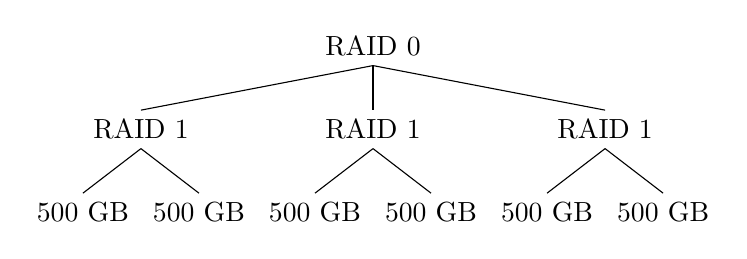
\begin{tikzpicture}
    \Tree
    [.RAID~0
        [.RAID~1
            [.500~GB ]
            [.500~GB ]
        ]
        [.RAID~1
            [.500~GB ]
            [.500~GB ]
        ]
        [.RAID~1
            [.500~GB ]
            [.500~GB ]
        ]
    ]
\end{tikzpicture}
\end{center}


\begin{itemize}
    \item \textbf{Najszybszy zapis i odczyt}.
    \item \textbf{Odporność na błędy}.
    \item \textbf{Wykorzystuje} efektywnie \textbf{50\%} pojemności całkowitej.
    \item Najlepszy, ale najdroższy.
\end{itemize}

\subsection{RAID 01 (0+1)}
RAID 1 złożony z RAIDów 0 (zamiast dysków).
RAID 0+1 jest uważany za \textbf{gorszy} niż RAID 10.
RAID 0+1 \textbf{nie przetrwa dwóch równoczesnych
awarii} jeśli \textbf{nie} są to dyski \textbf{z tego samego układu} RAID. Po awarii jednego dysku, \textbf{wszystkie dyski} w drugim pasku stanowią \textbf{krytyczne punkty}. \textbf{Połowa} dysków \textbf{przestaje być wykorzystywana}.

\begin{center}
    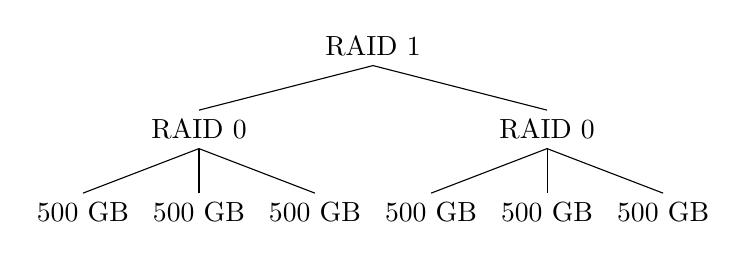
\begin{tikzpicture}
    \Tree
    [.RAID~1
        [.RAID~0
            [.500~GB ]
            [.500~GB ]
            [.500~GB ]
        ]
        [.RAID~0
            [.500~GB ]
            [.500~GB ]
            [.500~GB ]
        ]
    ]
\end{tikzpicture}
\end{center}


\subsection{Zastosowanie systemów RAID}
\begin{itemize}
    \item \textbf{Dziennik transakcji} na oddzielnych systemach \textbf{RAID 1} lub \textbf{RAID 10}
    \item \textbf{Dane} powinny być umieszczone w systemach \textbf{RAID 5} (jeśli co najwyżej 10\% liczby wszystkich operacji to operacje zapisu) lub \textbf{RAID 10} (w przeciwnym przypadku).
    \item Należy dodać odpowiednią liczbę dysków aby \textbf{zapewnić co najwyżej 125 losowych op/s} na dysk. Należy systematycznie \textbf{monitorować liczbę operacji} na sekundę dla \textbf{każdego} dysku.
    \item Użycie systemu RAID \textbf{nie powinno zastąpić} odpowiedniej strategii robienia \textbf{kopii zapasowych}.
\end{itemize}

\section{Indeksy}
\begin{itemize}
    \item Indeksy odgrywają \textbf{kluczową rolę dla wydajności} w systemach baz danych.
    \item Cel stosowania: \textbf{zmniejszenie czasu szukania}, \textbf{zminimalizowanie liczby odczytów} z dysku.
    \item Mogą \textbf{zmniejszyć czas wykonania kwerend}. \item Mogą \textbf{wydłużać} czas wykonania operacji \textbf{zmiany} danych, jeśli zmiany te dotyczą \textbf{kolumny indeksowanej} co może powodować \textbf{konieczność} wykonania odpowiedniej \textbf{zmiany w indeksie}.
    \item Informacje na temat indeksów wraz z informacjami o wartościach przechowywanych w kolumnach (\textbf{statystyki}) są \textbf{analizowane} przez \textbf{optymalizatory kwerend} w celu wyznaczenia \textbf{najlepszego planu wykonania kwerendy}.
     \item Indeks \textbf{może ulegać fragmentacji}, zatem może wymagać okresowej \textbf{defragmentacji} lub \textbf{przebudowy}. Należy zadbać o \textbf{aktualizację statystyk}.
     \item \textbf{Obciążenie serwera} powinno być okresowo \textbf{monitorowane} m.in. w celu \textbf{dobrego indeksowania}.
\end{itemize}

\subsection{Typy indeksów dla plików sekwencyjnych}
\textbf{Indeksy dla plików sekwencyjnych}:
\begin{itemize}
    \item \textbf{Główne} (Primary) - na identyfikatorach wierszy.
    \item \textbf{Drugorzędne} (Secondary) - pomocnicze.\\
    
    \item \textbf{Proste}.
    \item \textbf{Złożone}.\\
    
    \item \textbf{Gęste} (zagęszczone, dense) – każdy wiersz danych ma swój wpis w indeksie.
    \item \textbf{Rzadkie} (niezagęszczone, sparse) – np. każdy blok danych ma jeden wpis w indeksie. Dane muszą być \textbf{posortowane według klucza indeksu} (może to być klucz główny w tabeli lub inne pola).\\
    
    \item \textbf{Grupujące} (clustering) – ten termin jest wieloznaczny. W odniesieniu do plików sekwencyjnych oznacza grupowanie w jednym bloku \textbf{wierszy z taką samą wartością klucza indeksu}; taki \textbf{indeks} budowany jest \textbf{na polu niekluczowym} i wymaga \textbf{posortowania wierszy} według \textbf{pola indeksowanego}.
    \item \textbf{Wielopoziomowe}.
\end{itemize}
\hfill \\
\textbf{Indeksy dla standardowych typów danych}:
\begin{itemize}
    \item Drzewa B+
    \item Tablice haszujące
    \item Indeksy binarne (mapy binarne)
\end{itemize}

\textbf{Indeksy dla danych przestrzennych, wielowymiarowych}:
\begin{itemize} 
\item Drzewa ćwiartek (quad trees), 
\item R-drzewa, 
\item k-d drzewa, 
\item indeksy binarne,
\item uogólnione haszowanie: pliki siatkowe, podzielone funkcje haszujące
\end{itemize}

\subsection{Drzewa B+}
\begin{itemize}
    \item \textbf{Wszystkie wartości w liściach}
    \item Każdy \textbf{wewnętrzny węzeł} (nie liść) drzewa B+ ma postać: \\
    $<P_1, K_1, P_2, K_2, \dots , P_{q-1}, K_{q-1}, P_q>$
gdzie $q<=p, P_i (i=1,...,q)$ jest wskaźnikiem do poddrzewa.\\
$K_1 < K_2 < \dots < K_{q-1}$.
    \item Dla każdej \textbf{wartości} X w poddrzewie wskazywanym przez $P_i$, mamy: $K_{i-1} < X <= K_i$ dla $1 < i < q$ oraz $X <= K_i$ dla $i = 1$ oraz $K_{i-1} < X$ dla $i = q$.
    \item Każdy \textbf{wewnętrzny węzeł} ma \textbf{co najwyżej p} wskaźników do poddrzew.
    \item Każdy \textbf{węzeł}, z wyjątkiem korzenia, ma \textbf{przynajmniej $\left \lceil p/2 \right \rceil$} wskaźników do poddrzew. 
    \item \textbf{Korzeń} ma \textbf{co najmniej dwa} wskaźniki do poddrzew, jeśli jest węzłem wewnętrznym.
    \item Węzeł wewnętrzny z q wskaźnikami, $q <= p$, ma \textbf{$q-1$ wartości}.
    \item Każdy \textbf{liść} drzewa B+ ma postać:\\ $<<K_1,P_{r_1}>, < K_2,P_{r_2} >, \dots , < K_{q-1},P_{r_{q-1}} >,P_{next}>>$, gdzie $q <= p$ i $P_{r_i}$ jest wskaźnikiem do danych, $P_{next}$ wskazuje następny węzeł liść (\textbf{liście tworzą listę}).\\
    $K_1 < K_2 < \dots < K_{q-1}, q <= p.$
    \item Każdy $P_{r_i}$ jest wskaźnikiem do danych, który wskazuje na:
    \begin{itemize}
        \item \textbf{rekord}, którego wartość w polu indeksowanym jest równa $K_i$\\
        lub 
        \item \textbf{blok} zawierający rekord\\
        lub 
        \item \textbf{blok} wskaźników do rekordów z takimi samymi wartościami $K_i$, jeśli klucz indeksu nie jest unikalny
    \end{itemize}
    W praktyce w SZBD unikalność może być zapewniona np. przez rozszerzenie klucza – dołączenie do klucza jakiejś liczby).
    \item Każdy węzeł liść przechowuje co najmniej $\left \lceil p/2 \right \rceil$ wartości.
    \item Wszystkie \textbf{węzły liście są na tym samym poziomie}.
\end{itemize}

\subsubsection{Operacje na drzewach B+}
\begin{itemize}
    \item \textbf{Podział liścia}
    \begin{itemize}
        \item Jeśli węzeł jest \textbf{pełny} i ma być do niego wstawiony nowy wpis, wówczas węzeł zostaje \textbf{podzielony}.
        \item Pierwsze $j = \left \lceil ((p\_leaf + 1)/2) \right \rceil$ wpisów \textbf{zostaje w oryginalnym} węźle, pozostałe zostają \textbf{przesunięte} do nowego węzła liścia. p\_leaf oznacza maksymalną liczbę wskaźników do danych w węzłach liściach.
        \item j-ta wartość jest \textbf{kopiowana do węzła rodzica} i węźle tym tworzony jest \textbf{nowy wskaźnik} (do nowego węzła).
    \end{itemize}
    \item \textbf{Podział węzła wewnętrznego}
    \begin{itemize}
        \item Jeśli węzeł wewnętrzny jest \textbf{pełny} i ma być do niego wstawiony nowy wpis, wówczas węzeł \textbf{zostaje podzielony}.
        \item Wpisy aż do $P_j$ – j-tego wskaźnika do poddrzewa, gdzie $j= \left \lceil ((p+1)/2) \right \rceil$ \textbf{są zatrzymane}, podczas gdy wartość j-ta jest \textbf{przesuwana} do \textbf{węzła macierzystego}, nie kopiowana.
        \item \textbf{Nowy węzeł} wewnętrzny przechowuje wpisy od $P_{j+1}$.
        \item Podział może \textbf{propagować w górę} aż do utworzenia \textbf{nowego węzła korzenia}.
    \end{itemize}
    \item \textbf{Usuwanie wartości}
    \begin{itemize}
        \item Usunięcie wartości jest \textbf{zawsze realizowane w liściu}, jeśli usunięta wartość występuje również w węźle wewnętrznym, musi być też stamtąd usunięta.
        \item Przy usuwaniu $K_i$ z \textbf{węzła wewnętrznego}, wartość $K_{i-1}$ umieszczona bezpośrednio z lewej strony usuwanej wartości w \textbf{liściu} musi \textbf{zastąpić wartość $K_i$} w węźle wewnętrznym.
        \item Usuwanie wpisów może doprowadzić do \textbf{zmniejszenia liczby wpisów w węźle poniżej wymaganego z definicji poziomu}. W tym przypadku \textbf{wpisy z sąsiadów} są rozmieszczane tak, by węzły były \textbf{wypełnione w odpowiednim stopniu}. Jeśli nie da się tego zrealizować, wówczas \textbf{sąsiadujące węzły są łączone} i \textbf{liczba liści zostaje zmniejszona}.
    \end{itemize}
\end{itemize}

\subsubsection{Indeksy typu drzewa B+}
Wiele systemów umożliwia \textbf{wybór współczynnika wypełnienia węzłów} (PCTFREE w Oracle), a nawet można ustawiać współczynnik wypełnienia \textbf{osobno dla liści}, \textbf{osobno dla węzłów wewnętrznych} (FILLFACTOR i PADINDEX w systemie MS SQL Server).\\
\textbf{Indeksy z odwróconym kluczem} - wartość klucza jest zmieniana, np. \textbf{zapis binarny jest negowany}. W pewnych przypadkach \textbf{zapobiega} to \textbf{powstaniu wąskiego gardła}, jeśli więcej transakcji odwołuje się do \textbf{podobnych wartości klucza} (znajdujących się w jednym bloku).\\

\textbf{Fragmentacja indeksów typu drzewo B+}\\
\textbf{Wstawianie} nowych wartości klucza może spowodować
\textbf{konieczność podziału węzła}. Przy podziale 50+50 i
niekorzystnym układzie danych, po wykonaniu pewnej liczby
wstawień \textbf{większość węzłów może być uzupełniona tylko w 50\%}. \textbf{Nowo} przydzielone węzły (bloki) mogą być \textbf{rozrzucone po dysku} (nie są sąsiadujące).\\

\textbf{Defragmentacja indeksów} - \textbf{zmiana kolejności} bloków (stron), przebudowa z \textbf{przywróceniem oryginalnego} lub \textbf{ustawieniem nowego współczynnika wypełnienia} węzłów (może być oddzielnie dla węzłów liści i dla poziomów nieliściastych). \\

\textbf{Charakteryzacja indeksów typu drzewa B+}
\begin{itemize}
    \item \textbf{selektywność} - liczba różnych wartości klucza (wartość względna, liczba różnych wartości podzielona przez liczbę wierszy),
    \item \textbf{dane} dotyczące \textbf{fragmentacji} bloków i ekstentów (liczba bloków i ekstentów ułożonych \textbf{nie po kolei}, \textbf{średnie zapełnienie} bloku)
    \item \textbf{współczynnik zgrupowania} (clustering factor) – liczba bloków, przez które należy przejść przy skanowaniu wierszy indeksu.\\ 
    Przy indeksie \textbf{zgodnym z posortowaniem} wierszy jest to \textbf{liczba bloków} danych; przy indeksie \textbf{niezgodnym}  oraz przy \textbf{dużych wierszach} liczba ta może być \textbf{bliska liczbie wierszy}.
    \item \textbf{statystyki} (mogą zawierać histogramy), mogą być budowane \textbf{również dla kolumn nie indeksowanych}; tworzone i modyfikowane automatycznie lub ręcznie na podstawie pewnej próby.
\end{itemize}


\subsection{Sposoby przechowywania danych w plikach}
\begin{itemize}
    \item \textbf{Sterty} (heap) – \textbf{nieuporządkowane}, zapis w blokach (stronach).
    \item \textbf{Tablice o strukturze indeksowej} (IOT Index Organized Tables, Oracle), \textbf{indeksy grupujące} (Clustered Indexes, MS SQL Serwer).
    \item \textbf{Klastry} (clusters) – przechowywanie \textbf{dwóch lub więcej} tabel w \textbf{jednym pliku}, wiersze są \textbf{posortowane} według pola (pól) łączącego.
\end{itemize}
\hfil \\
\textbf{W MS SQL Server}\\
Można budować \textbf{indeksy grupujące} na polach \textbf{innych niż klucze}.\\
\textbf{Indeksy niegrupujące} (niezgrupowane, non-clustered) mają \textbf{inną budowę} węzłów liści w \textbf{przypadku}, gdy dla tabeli \textbf{istnieje już indeks grupujący}. Zamiast wskaźników do wierszy przechowywane są \textbf{wartości klucza indeksu grupującego}. \textbf{Zaleta}: w przypadku \textbf{zmiany położenia wiersza} (np. po podziale strony)
\textbf{nie trzeba modyfikować} indeksów niegrupujących.\\

\textbf{IOT w Oracle}\\
\textbf{Secondary indexes} (odpowiednik indeksów niegrupujacych w SQL Serwerze): odnajdywanie wiersza na podstawie \textbf{wartości guess} tzn. wykorzystanie physical ROWID, a w przypadku gdy wiersz nie zostanie znaleziony wykorzystanie logical ROWID. W IOT \textbf{wiersze mogą być podzielone pionowo}: \textbf{część} kolumn jest przechowywana w \textbf{liściach} IOT, \textbf{część} może być przechowywana w oddzielnych \textbf{blokach}. 
\end{document}
